
%
% # INTRODUCTION:
%
% This write up is for Lab3: Logic Implementation Using IC's
%
% Specifically this was used for the class Logic Design Fundamentals (EECE 144)
% taught by Kurtis Kredo [http://www.ecst.csuchico.edu/~kkredo/]
% during the Fall 2011 semester at CSU Chico [www.csuchico.edu].
% 
% ## LaTeX
%
% This file is written for LaTeX [http://www.latex-project.org/]
% which is used to process this file in to a completely formatted
% document.
%
% If you are unfamiliar with LaTeX it can seem daunting at first
% (as with anything new) but there are many benefits.
% Imagine writing a document in Word except without
% having to worry about the tedious things such as line breaks,
% indentation, table of contents, appendices, font styles,
% heading sizes, citations/references, page numbers.
% LaTeX lets you focus on the content without
% worrying about the tedious details.  It is also excellent for
% producing mathematical formulas.
% 
% If you are collaborating with someone else you can simply edit
% the sections and paragraphs in this file as needed.
%
% To process this file use a command such as 'rubber'.
%
%   bash$ rubber skel.tex
%   (output to skel.dvi)
%   bash% rubber --pdf skel.tex
%   (output to skel.pdf)
%
% # AUTHORS (of this template):
%
%   Jeremiah Mahler <jmmahler@gmail.com>
%   https://www.google.com/profiles/jmmahler#about 
%
% # COPYRIGHT:
%
%   Copyright (C)  2011 Jeremiah Mahler <jmmahler@gmail.com>.
%   Permission is granted to copy, distribute and/or modify this document
%   under the terms of the GNU Free Documentation License, Version 1.3
%   or any later version published by the Free Software Foundation;
%   with no Invariant Sections, no Front-Cover Texts, and no Back-Cover Texts.
%   A copy of the license is included in the file "fdl-1.3.txt".
%

\documentclass[12pt]{article}
%\documentclass[10pt]{article}

%\usepackage{mslapa}
\usepackage{hyperref}
\usepackage{amsmath}
\usepackage{graphicx}
\usepackage{ulem}
%\usepackage{vmargin}
\usepackage{tabularx}
\usepackage{sectsty}
\usepackage{pbox}
\usepackage{bigstrut}
\usepackage{enumerate}

%\usepackage{cleveref}

%\setpapersize{USletter}
\sectionfont{\normalsize}
\subsectionfont{\normalsize}

% configure \bigstrut size
% This configures spacing above and below rows in a tabularx.
%\renewcommand{\bigstrutjot}{6pt}
\renewcommand{\bigstrutjot}{2.0\jot}

\setlength{\parindent}{0in}

\raggedright

\begin{document}

% {{{ Cover Page

\centerline{\bf EECE 144}
\centerline{\bf Fall 2011}
\centerline{\bf}
\centerline{\bf Lab Report \#3}
\centerline{\bf Section 4}
\centerline{\bf 9/21/2011}

% signature area
\begin{center}
\begin{tabularx}{\textwidth}[b]{X l l}
Submitted by: & & \\
Signature & Printed Name & Date \\
\hline
\multicolumn{1}{|X|}{} & \multicolumn{1}{|l|}{\bigstrut \bf Jeremiah Mahler} & \multicolumn{1}{|l|}{\bf Sep 21, 2011} \\
\hline
\multicolumn{1}{|X|}{} & \multicolumn{1}{|l|}{\bigstrut \bf Marvanee Johnson} & \multicolumn{1}{|l|}{\bf Sep 21, 2011} \\
\hline
\end{tabularx}
\end{center}
% }}}

\section{Description/Objectives}

The objective of this lab is to implement a logic function
using actual hardware.
The basic interfacing circuits using switches and outputs
using LEDs are also introduced.

\section{Procedure}

Equation \ref{eq:fn1} will be used as the logic function for this lab.
The first step is to build a truth table definition (Figure \ref{fig:out1}).
The next step is to implement the logic function using Logisim \cite{LOGISIM}.
This will help as a guide for connecting hardware and can also be used
to verify the truth table in Figure \ref{fig:out1}.
The chips being used only have two inputs so the gates in Logisim should
also use only two inputs.

\nocite{LOGISIM}

\begin{align}
& a c + a' b + a b' c' \label{eq:fn1}
\end{align}

\begin{figure}[!hbt]

\center

\begin{tabular}[t]{| l | l | l | l |}
\hline
\multicolumn{4}{| c |}{$a c + a' b + a b' c'$} \\
\hline
$a$ & $b$ & $c$ & z (out) \\
\hline
0 & 0 & 0 & 0 \\
\hline
0 & 0 & 1 & 0 \\
\hline
0 & 1 & 0 & 1 \\
\hline
0 & 1 & 1 & 1 \\
\hline
1 & 0 & 0 & 1 \\
\hline
1 & 0 & 1 & 1 \\
\hline
1 & 1 & 0 & 0 \\
\hline
1 & 1 & 1 & 1 \\
\hline
\end{tabular}

\caption{Truth table of outputs for the function $a c + a' b + a b' c'$.}
\label{fig:out1}
\end{figure}

\begin{figure}[!hbtp]
\center
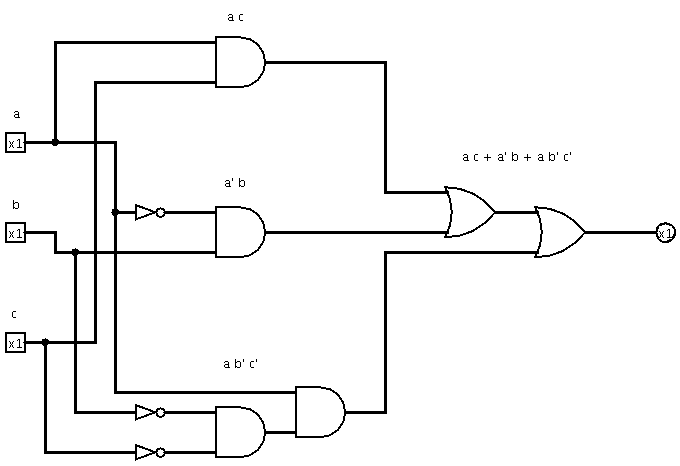
\includegraphics[scale=0.5]{Lab3-circuit}
\caption{Logic circuit $a c + a' b + a b' c'$ defined in Logisim.}
\label{fig:logisim1}
\end{figure}

%\clearpage

The inputs to the chips will be in the form of mechanical switches.
If the switch is connected from the source voltage (5 volts) to the
chip it will read the high value correctly but it will not read low
correctly because the open circuit is not equivalent to low. 
To remedy this issue a pull down resistor is used to connect the
pin at the chip to ground.
A 1k resistor works well for this, larger values such as 10k may not
work properly.

The outputs from the chips will be used to drive a LED.
For the LEDs used in this lab the current should be approximately
20 mA if we assume that the diode behaves as a short with no voltage drop.
Using Ohm's Law ($V = i \cdot R$) and a source voltage of 5 volts
this results in a resistor of 250 ohms.
Select the resistor nearest to this value or larger.

% TODO - hardware circuit

\section{Observations}

%\clearpage

\section{Conclusion}

% flush all the figures
%\clearpage

%\pagebreak
\renewcommand*{\refname}{\vspace{-8mm}}
\section{References}
%\bibliographystyle{plain}
%\bibliographystyle{mslapa}
\bibliographystyle{ieeetr}
\bibliography{../references}

% Appendix (if needed)

\end{document}

% vim:foldmethod=marker
